\chapter{Transfer Learning in One Class CF for Shopping Prediction}
\label{chp:trimf}
\section{Problem Settings}
\subsection{Background}
\par{
In real-world, a person usually has different kinds of behaviors before buying one thing. For online shopping sites, their goal is to let users buy their products, but the user-item matrix for deal is extremely sparse( less than $0.001\%$ ). Therefore, if we only use the available information, we cannot achieve a reliable or even reasonable performance.

In an online shopping site, there are two main actions - click and purchase. Both can form a matrix which consists of only binary data(1-action happened, 0-unknown). Let's denote $X_d$ to be the matrix of deal, $X_c$ to be the matrix of click. We know that deal matrix $X_d$ is very sparse and although click matrix $X_c$ is also sparse, it is much denser than $X_d$. To use more data, we develop a transfer learning algorithm(TRIMF) that leverages click data to predict purchasing. Compared with former methods which only share either rating patterns or latent features , our method shares both rating patterns and latent features through cluster-level transformation and overlapping matrices. Experiments in \ref{sec:offline} show that our algorithm performs better than other baseline(transfer and non-transfer) methods.}

\subsection{Problem Definition}
  \begin{itemize}
  \item Input: [0-1 matrix:user click matrix $X_C(m_c*n_c)$, user deal matrix $X_d(m_d*n_d)$] , $m_c, m_d$ denote the number of users, $n_c, n_d$ denote the number of items. Users and items partially overlap.
  \item Output: Two prediction matrix $P_C(m_c*n_c), P_d(m_d*n_d)$, which predict users' purchasing behavior.
  \end{itemize}



\section{TRIMF}
\subsection{Weighting Scheme of TRIMF}
  \par{Former one-class CF methods ~\cite{4781121}, ~\cite{4781145} use weighted low-rank approximation to tackle the problem that all observed ratings are 1. Given a rating matrix $R = (R_{ij})_{m*n} \in \{0, 1\}^{m*n}$ with $m$ users and $n$ items and a corresponding non-negative weight matrix $W = (W_{ij})_{m*n} \in R^{m*n^+}$ , weighted low-rank approximation aims at finding a low rank matrix $X = (X_{ij})_{m*n} $minimizing the objective of a weighted Frobenius loss function as follows : $L(X) = \|\sum W_{ij}(R_{ij} - X_{ij})\|_2$. 

In ~\cite{4781121}, the authors consider actions that happen more than once(e.g. multiple clicks on an item). Negative entries are ignored; for each positive entry, its weight is proportional to its frequency, since higher frequency can mean that we are more confident about the entry. For example, user $i$ viewed item $j$, $n$ times, then $W_{ij} = 1 + log(n)$. In ~\cite{4781145}, positive entries all have same weight 1, while negative entries are considered differently. According to their experiments, the user-oriented weighting scheme can achieve the best performance. That is, for negative entries $W_{ij} \propto \sum_j{R_{ij}}$, the idea is that if a user has more positive examples, it is more likely that the user does not like the other items, that is, the missing data for this user is negative with higher probability.

In our method, we adopt these weighting schemes to give missing values proper weights, that is, for positive entries we use the weighting scheme in ~\cite{4781121} and for negative entries we use user-oriented weighting. $$ W_{ij}=\left\{
\begin{aligned}
1 + log(n) & & X_{ij} = 1\\
log(\sum_j{R_{ij}}) &  & X_{ij} = 0 \\
\end{aligned}
\right.
$$}
\subsection{Transfer Learning in TRIMF}

Usually users' deal data is very sparse. For instance, users will buy $n_d$ items in one day while clicking $n_c$ items which often results in $n_d \ll n_c$. Therefore, only using deal data is not sufficient. Traditional transfer learning methods use matrix factorization and share a certain part of low-rank matrices to achieve knowledge transfer(e.g. user-latent factor, rating pattern). However, none of them apply the selective-sharing scheme as ours does.

In TRIMF, rating matrices are factorized into three parts : $X = USV^T$. The first part $U$ stands for user clustering results or latent factor, $V$ stands for item clustering results or the latent factor, while $S$ stands for the clustering relationships between user clusters and item clusters. We want to learn a better cluster-level rating pattern $S$ from users' deal data with the help of users' click data, not just use users' deal data. Therefore we factorize two matrices $X_c, X_d$ together. In order to transfer knowledge, we must make sure that their latent spaces are the same. For a user who has click and deal actions, it would be particularly beneficial that his latent vectors factorized from $X_c, X_d$ are the same.

Therefore, for overlap users and items, we want their clustering vector  $U,V$ to be the same. What is more, we want even more knowledge transfer from the matrix $S$ which stands for cluster relationship or rating patterns. However, what a user likes to click is not always the item he wants to buy. In Yixun, there are only two common items in the top 10 click items and top 10 purchase items (Table ~\ref{tbl:topitem}). Therefore these rating patterns should somehow be related but not the same. We cannot simply make the pattern matrix $S$ the same in the prediction. 

\begin{table}[h]

%\begin{Large}
\label{tbl:topitem}
\begin{center}
\begin{tabular}{| c | c |}
\hline
Top click items & Top purchase items \\
\hline
Iphone 5s & Tissue\\
Xiaomi 3 & Laundry soap powder\\
Thinkpad & Xiaomi 3\\
CPU & Snacks\\
Hard disk & Battery\\
Router & Iphone 5s\\
Earphone & Mouse\\
\hline
\end{tabular}
\caption{Top 10 click items and purchase items in Yixun.}
\end{center}
%\end{Large}
\end{table}

\par{After careful observation we found that there are some items which belong to the same category with a higher conversion rate (user tends to buy after clicking), but not with other categories. There are also some users who like window-shopping while others buy an item straight after clicking. These are all cluster-level features. We design a mapping function to allow the learnt $S$ better suit the data.

We design two mapping vectors: $U,V$, if we have learnt a rating pattern $S_c$ from a click matrix, then for the deal matrix pattern we have $S_d^{ij} = U_i * S_c^{ij} * V_j$. The transformation is based on $S_c$ to enable knowledge transfer, while after being multiplied by $U$ and $V$ we can capture the difference between them, at the cluster-level. }

\subsection{Object Function}
\par{We use a weighted non-negative matrix tri-factorization method to deal with the problem as illustrated below. 
\begin{figure}

%\begin{Large}

\begin{center}
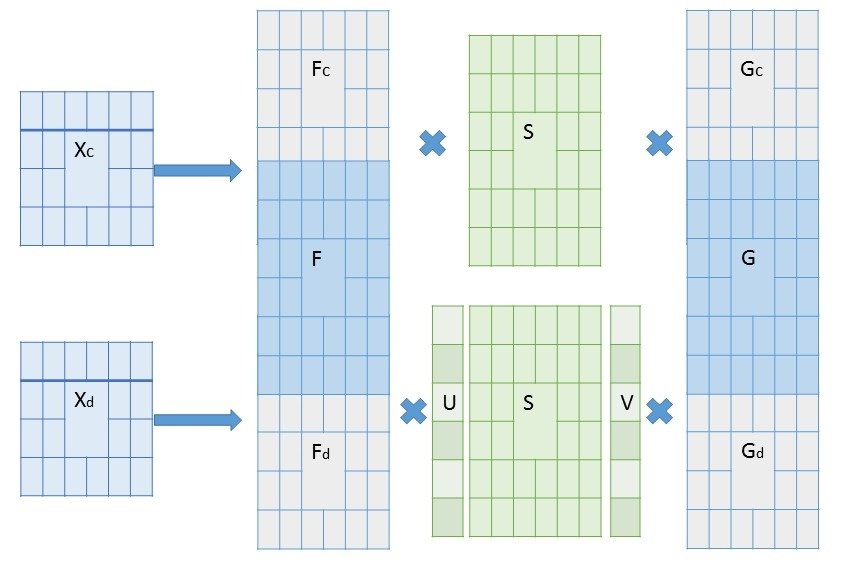
\includegraphics[width=400px]{fig/trimf.jpg} 
\caption{Graphical model of TRIMF.}
\label{fig:trimf}
\end{center}
\end{figure}}
 
  \par{Objective Function:$$min_{F,G,S,U,V} W_c\odot ||X_c - (F;F_c)S(G;G_c)'||_2 + W_d\odot ||X_d - (F;F_d)(USV)(G;G_d)'||_2 $$}

  \par{
    \begin{itemize}
    \item $W_c,W_d$ are the weights for $X_C, X_d$, every observed entry has weight $1 + log(frequency)$. While others have weight $W_{ij} = \sum_jI({R_{ij}})$.
    \item $F, G$ are the soft clustering result matrices for overlapped users(items), they are forced to be the same. $F_c,F_d,G_c,G_d$ are matrices for unique users(items).
    \item $U,V$ are two diagonal matrices, $U_{ii}$ scales every $S_{i*}$ to $U_{ii}S_{i*}$, and models the users' cluster-level transformation from click to deal. While $V_{jj}$ scales every $S_{*j}$ to $S_{*j}V_{jj}$, it models the items' cluster-level transformation from click to deal.
    \item When predicting, we use $(F;F_d)(USV)(G;G_d)$ to predict users who have deal data. Then since we got two mapping matrices $U,V$, we apply $U,V$ back to the click pattern matrix $S$ to predict for users who have click data, i.e. we use $(F;F_c)(USV)(G;G_c)$.
    \end{itemize}
}



\begin{section}
  {Solution to TRIMF \& Algorithm}
\par{Following the update rules in ~\cite{Zhuang:2011:EAW:1952191.1952195}, we use an alternately iterative algorithm to solve the objective function.}

Firstly, we declare some denotations:
\begin{itemize}
	\item $Ic,Icc,Icd,Id$ : $(Ic,Icc)*(F;F_c) = I*(F;F_c)$ and $(Icd,Id)*(F;F_d) = I*(F;F_d)$
	\item $sg$ : $S*G'*G*S'$
	\item $F_1, F_2$ : $[F;F_c]$, $[F;F_d]$
\end{itemize}
\par{In each round of iterations these matrices are updated as :
$$F \leftarrow F .* \sqrt{\frac{Icc'*(W_c.*X_c)*G*S' + Icd'*(W_d.*X_d)*G*S'}{(Icc'*Icc*F + Icc'*Ic*F_c + Icd'*(Icd*F + Id*F_d))*sg)}}$$
$$F_c \leftarrow F_c .* \sqrt{\frac{Ic'*(W_c.*X_c)*G*S'}{Ic'*(Icc*F + Ic*F_c)*sg}}$$
$$F_d \leftarrow F_d .* \sqrt{\frac{Id'*(W_d.*X_d)*G*S'}{Id'*(Icd*F + Id*F_d)*sg }}$$
$$G \leftarrow G .* \sqrt{\frac{W_c.*X_c*F_1*S + (W_d.*X_d)'*F_2*S}{(G*(S'*F_1'*F_1*S + S'*F_2'*F_2*S)}}$$
$$U \leftarrow U .* \sqrt{\frac{F_2'*(W_d.*X_d)*G*V'*S'}{F_2'*F_2*U*S*V*G'*G*V'*S'}}$$
$$V \leftarrow V .* \sqrt{\frac{S'*F_2'*(W_d.*X_d)*G}{S'*F_2'*F_2*S*V*G'*G}} $$



}

\par{The user-item matrix is typically very sparse with $z \ll nm$ non-zero entries while $k$ is also much smaller than n, m. Through using sparse matrix multiplications and avoiding dense intermediate matrices, the update steps can be very efficiently and easily implemented. In particular, updating F, S, G each takes $O(k^2 (m + n) + kz)$ , and the algorithm usually reaches convergence in less than 200 iterations.}

\begin{algorithm}[tb]
\caption{Algorithm for TRIMF.}
\begin{algorithmic}

\STATE {\bfseries Input:} $\X_{c}$, $\X_{d}$\\
$\X_{c} \in \mathbb{R}^{m_c\times n_c}$: the purchase data \\
$\X_{d} \in \mathbb{R}^{m_d\times n_d}$: the click data\\

\STATE {\bfseries Initialize:} Initialize $W_c, W_d$ : $(1+log(freq))$ for observed, $\sum_jI({R_{ij}})$ for unseen, $F,G,S,U,V$ : $random$, Set overlap numbers for users and items

\FOR{ $i$ = 1 to $T$}

\STATE update $F$

\STATE update $F_c$, $F_d$

\STATE  update $G$

\STATE  update $S$

\STATE  update $U, V$


\ENDFOR

\STATE {\bfseries Output:} $F,G,S,U,V$

\end{algorithmic}
\label{algorithm:TRIMF}
\end{algorithm}

\end{section}
